%%%%%%%%%%%%%%%%%%%%%%%%%%%%%%%%%%%%%%%%%%%%%%%%%%%%%%%%%%%%%%%%%%%%%%%%%%%%%%%%
%%                                                                
%%      SWSC LaTeX class for Journal of Space Weather and Space Climate
%%      
%%                                      (c) Springer-Verlag HD
%%                                      revised by EDP Sciences
%%                                      further revised by J. Watermann 
%%
%%%%%%%%%%%%%%%%%%%%%%%%%%%%%%%%%%%%%%%%%%%%%%%%%%%%%%%%%%%%%%%%%%%%%%%%%%%%%%%%
%%
%%      This demonstration file was derived from aa.dem
%%  
%%      AA vers. 7.0, LaTeX class for Astronomy & Astrophysics
%%      demonstration file
%%                                                (c) Springer-Verlag HD
%%                                                revised by EDP Sciences
%%
%%%%%%%%%%%%%%%%%%%%%%%%%%%%%%%%%%%%%%%%%%%%%%%%%%%%%%%%%%%%%%%%%%%%%%%%%%%%%%%%
%%
%%      modified for Journal of Space Weather and Space Climate
%%      by Jurgen Watermann, Editorial Advisor to SWSC
%%
%%      01-04-2012 original version
%%      02-04-2012 revision 1
%%      12-07-2012 revision 2
%%      06-12-2012 revision 3 
%%      01-01-2014 revision 4
%%      05-03-2016 revision 5
%%      11-05-2018 revision 6  (equations and figure captions line numbered)
%%
%%%%%%%%%%%%%%%%%%%%%%%%%%%%%%%%%%%%%%%%%%%%%%%%%%%%%%%%%%%%%%%%%%%%%%%%%%%%%%%%
%%
%%      The two sub-figures referenced in this template are of eps and png type,
%%      respectively, in order to demonstrate the usepackages subfigure and
%%      epstopdf and thus create pdf-only output 
%%
%%      If you want to use TexLive or MikTex together with a bibtex bibliography 
%%      file you may run Latex2e from the command line 
%%          pdflatex -shell-escape swsc.tex
%%          bibtex swsc (do not include an extension such as .tex or .bib)
%%          pdflatex -shell-escape swsc.tex
%%          pdflatex -shell-escape swsc.tex
%%
%%      A double call to pdflatex after calling bibtex is necessary in order to
%%      set citations and references correctly and insure that foreward/backward  
%%      linkage (backref option) is properly applied
%%      If you use MikTex you may need to make a triple call to pdflatex
%%
%%      If you are using TexLive or MikTex but not a bibtex type of bibliography
%%      you may simply run Latex2e twice from the command line 
%%          pdflatex -shell-escape swsc.tex
%%          pdflatex -shell-escape swsc.tex
%%
%%%%%%%%%%%%%%%%%%%%%%%%%%%%%%%%%%%%%%%%%%%%%%%%%%%%%%%%%%%%%%%%%%%%%%%%%%%%%%%%
%%
%%   single column 12-point version for review
%%

%%  with traditional abstract
\documentclass[referee,a4paper,12pt,traditabstract]{swsc} 

%%  with structured abstract 
%\documentclass[referee,a4paper,12pt,structabstract]{swsc} 
\usepackage{graphicx}
\usepackage{txfonts}
\usepackage{subfigure}
\usepackage{epstopdf}
\usepackage[displaymath,mathlines]{lineno}
\usepackage[authoryear,round]{natbib}
\usepackage[backref]{hyperref}
\usepackage{url}
\usepackage{pdfpages}
%%    This version assumes using bibtex with the swsc bibliography style file
\bibliographystyle{swsc}
\usepackage[none]{hyphenat}
\hypersetup{colorlinks=true,citecolor=cyan,urlcolor=cyan,linkcolor=blue}
\usepackage[]{xcolor}
%%    This version assumes using bibtex with the swsc bibliography style file
\bibliographystyle{swsc}

\hypersetup{colorlinks=true,citecolor=cyan,urlcolor=cyan,linkcolor=blue}

%%%%%%%%%%%%%%%%%%%%%%%%%%%%%%%%%%%%%%%%%%%%%%%%%%%%%%%%%%%%%%%%%%%%%%%%%%%%%%%%%%%%%%%%%%%%%%%%
\definecolor{CASIIlightindago}{RGB}{60,100,120}
\definecolor{CASIIdarkyellow}{RGB}{188,161,54}
\definecolor{CASIIdarkgreen}{RGB}{75,85,50}
\definecolor{CASIIaliceblue}{RGB}{16,120,150}

\begin{document}

\begin{linenumbers}  

   \title{Tracking usability and progress across disciplines: Using AULs for software and hardware}

   
   \titlerunning{TRLs to AULs}

   \authorrunning{Alexa J. Halford}

   \author{A. J. Halford \inst{1} \and A. G. Burrell \inst{2}
          }

   \institute{1: NASA Goddard, Greenbelt MD, USA:
              \email{Alexa.J.Halford@nasa.gov} \\
2: US Naval Research Laboratory, Washington DC, USA: 
              \email{angeline.burrell@nrl.navy.mil}
}



  \abstract
 %% context heading (optional). leave {} empty if necessary  
   {We need to show these examples to convince ESA to use AULs}        %% replace by pair of curly brackets, {}, if structured abstract is selected
   

   \keywords{Tracking usability --
                Validation --
                Verification
               }

   \maketitle
%%
%%________________________________________________________________
Perhaps another title taken from an article in the innovation journal ("From NASA to EU: the evolution of the TRL scale in Public Sector Innovation"  The Innovation Journal: The Public Sector Innovation Journal, Volume 22(2), 2017, article 3.) - From NASA to the EU - The evolution of the TRL framework to the AULs. 


\section{The need for a generalized tracking system to work across project type}

\subsection{Why TRLs don't work for research or software projects}

Yes they can be shoe horned into the TRLs, but what is missing. TRLs are designed for tools that have a single purpose 

%%  This two-panel figure was inserted by JFW to demonstrate the subfigure and epstopdf packages

\subsection{Brief intro into the AULs}

The unique needs of the space weather community led to the modification of existing research-to-application communication frameworks to create the Application Usability Level (AUL) framework \citep{halford19}. Applying AULs to model and data analysis efforts can benefit space physics research. These benefits include improving access to collaborators, project transparency, and communication of project results. As the requirements and user interests for each application are unique, the AUL framework uses specifically-tuned metrics. 
   
   
   
\begin{figure}
\centering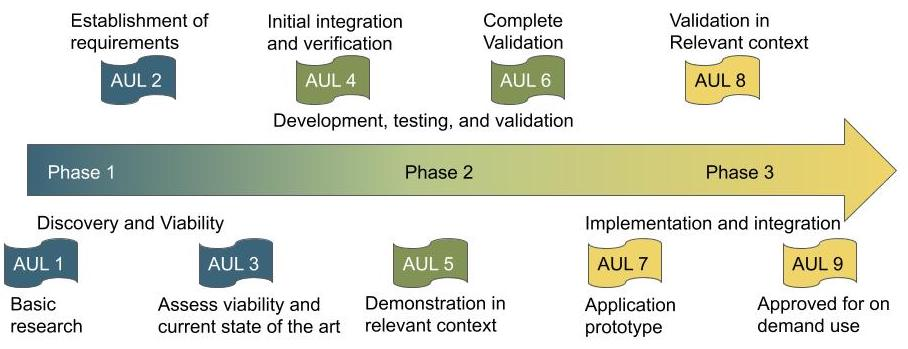
\includegraphics[width=0.9\linewidth]{Fig_AUL.jpg}
\caption{Application Usability Level (AUL) diagram. The progress of a project towards an application moves from AUL 1 to AUL 9, passing through three main phases: discovery, development, and implementation. Each of these are described in the main text. }\label{Fig_AUL}

\end{figure}



\begin{table}
\caption{A brief description of the AUL phases and levels}
\centering
\begin{tabular}{llll}\hline
Phase & Phase definition & AUL & Level description \\
 \hline
 & & \textcolor{CASIIaliceblue}{1}& \textcolor{CASIIaliceblue}{Basic research}\\
 \textcolor{CASIIaliceblue}{{\bf Phase 1} }& \textcolor{CASIIaliceblue}{{\bf Discovery and Viability }} & \textcolor{CASIIaliceblue}{2} & \textcolor{CASIIaliceblue}{Establishment of users and their requirements}\\ 
& & \textcolor{CASIIaliceblue}{3} &\textcolor{CASIIaliceblue}{Assess viability and current state of the art} \\
 \hline
 \hline
 & & \textcolor{CASIIdarkgreen}{4}& \textcolor{CASIIdarkgreen}{Initial integration and verification}\\
 \textcolor{CASIIdarkgreen}{{\bf Phase 2} }& \textcolor{CASIIdarkgreen}{{\bf Development, Testing,  }} & \textcolor{CASIIdarkgreen}{5} & \textcolor{CASIIdarkgreen}{Demonstration in the relevant context}\\ 
& \textcolor{CASIIdarkgreen}{{\bf and Validation}}& \textcolor{CASIIdarkgreen}{6} &\textcolor{CASIIdarkgreen}{Completed validation} \\
 \hline 
 \hline
 & & \textcolor{CASIIdarkyellow}{{7}}& \textcolor{CASIIdarkyellow}{{Application prototype}}\\
 \textcolor{CASIIdarkyellow}{{{\bf Phase 3}}}& \textcolor{CASIIdarkyellow}{{{\bf Implementation and Integration}}} & \textcolor{CASIIdarkyellow}{{8}} & \textcolor{CASIIdarkyellow}{{Validation in relevant context}}\\ 
& \textcolor{CASIIdarkyellow}{{{\bf into Operation}}} & \textcolor{CASIIdarkyellow}{{9}} &\textcolor{CASIIdarkyellow}{{Approved for on-demand use}} \\


\label{Tab_AUL}
\end{tabular}
\end{table}


\section{Definitions and terminology}

What terms are perhaps needed to be defined and/or are used differently by the Engineers, Software guys, and the research community. 


\section{Examples}
\subsection{At least one hardware, single instrument}

\subsection{At least one hardware - full project how the lowest of the instrument/system AULs providing the AUL for the entire project/mission/hardware etc.}

For doing a whole mission I think it is worth considering how AULs fit in with the NASA and ESA phases as well as TRLs. Should AULs cover the whole life cycle of the project? Or end at start of ops (like TRLs do)?

Borrowing (stealing) the Whale Chart from AFRL (\href{https://smartech.gatech.edu/bitstream/handle/1853/8034/SSEC_SD5_ppt.pdf}{AFRL link}) but adding the NASA Mission Phases (\href{https://solarsystem.nasa.gov/basics/chapter7-1)}{NASA Link}) and ESA Mission Phases (\href{(https://www.space.irfu.se/seminars/20180523-Cripps-HW_Project.pdf}{ESA link}) (not necessarily correctly...):

\begin{figure}[h!t]
    \centering
    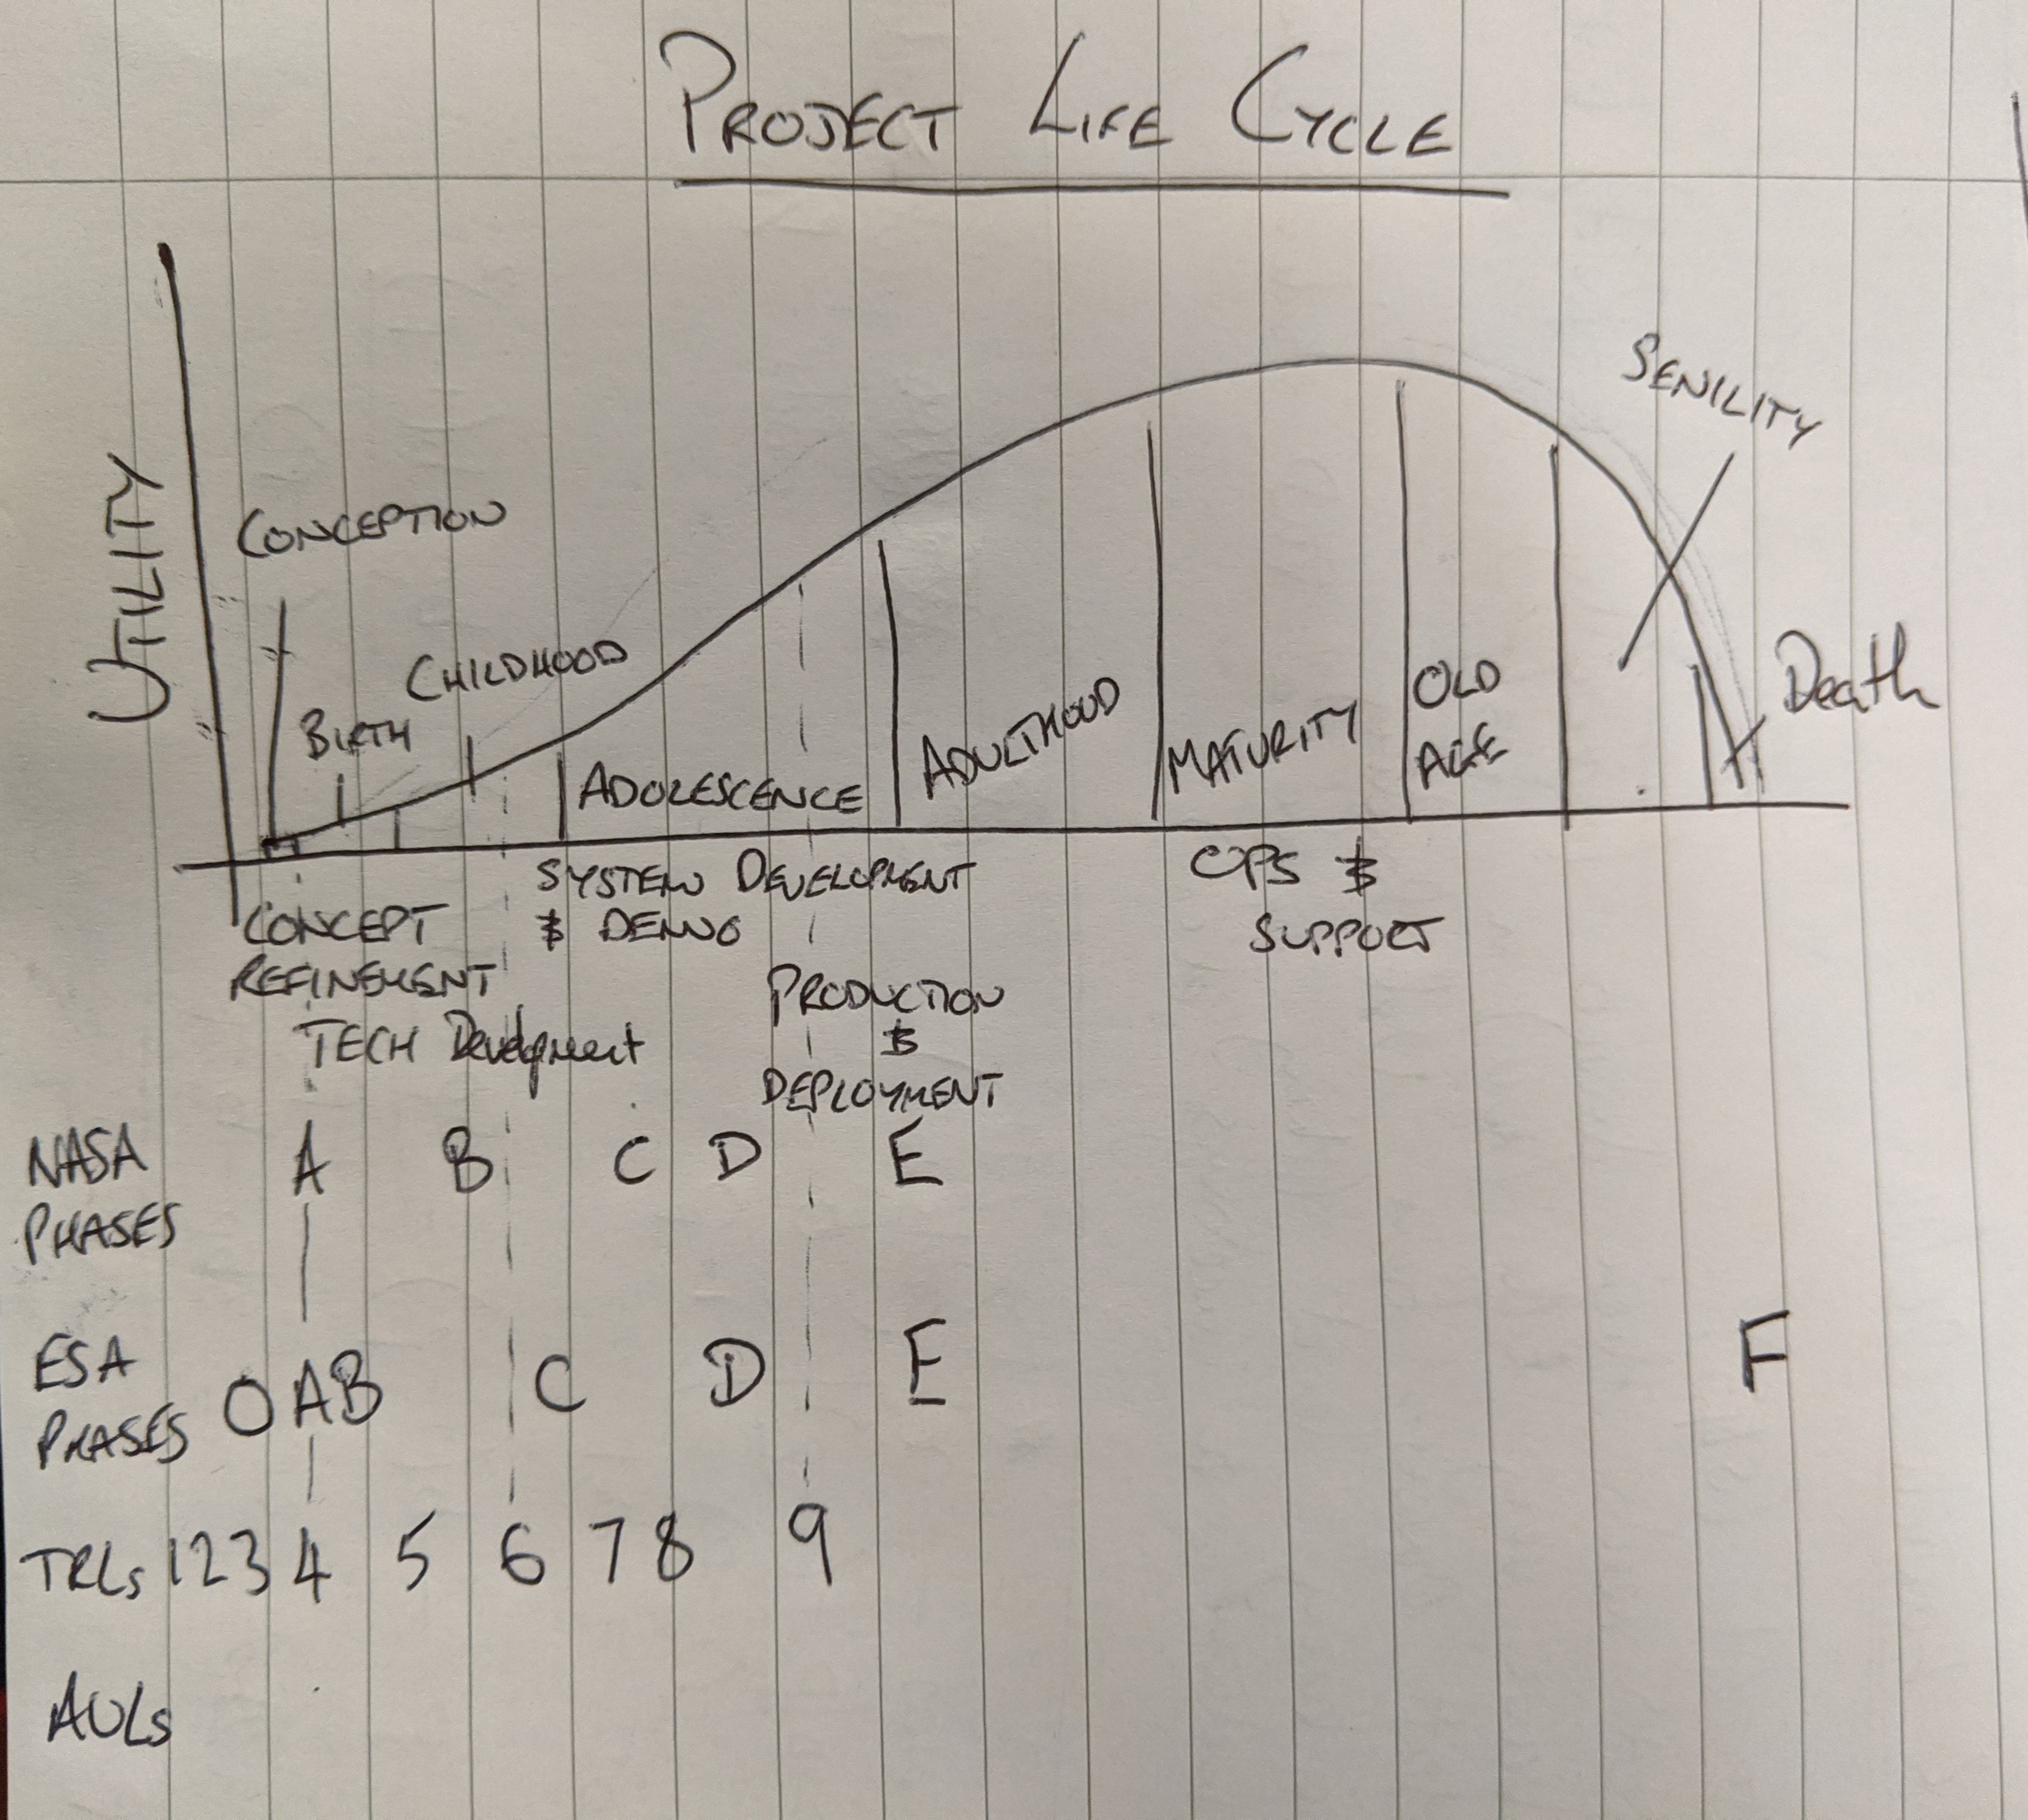
\includegraphics[scale=0.1]{whaleChart_hand.jpg}
    \caption{Hand drawn whale chart}
    \label{fig:whaleChart}
\end{figure}

\textit{To map between TRLs and AULs we'll need to have a list of the TRLs!}:
\textbf{TRL 1}
Basic principles observed and reported

Basic scientific research that can be turned into an application or a concept under a research and development program is considered.

\textbf{TRL 2}
Technology concept or application formulated

An idea is proposed for the practical application of current research, but there are no experimental proofs or studies to support the idea.

\textbf{TRL 3}
Concept or application proven through analysis and experimentation

Active research and development begins, including analytical laboratory-based studies to validate the initial idea, providing an initial "proof of concept."

\textbf{TRL 4}
Basic prototype validated in laboratory environment

Basic examples of the proposed technology are built and put together for testing to offer an initial vote of confidence for continued development.

\textbf{TRL 5}
Basic prototype validated in relevant environment

More realistic versions of the proposed technology are tested in real-world or near real-world conditions, which includes initial integration at some level with other operational systems.

\textbf{TRL 6}
System or subsystem model or prototype demonstrated in a relevant environment

A near final version of the technology in which additional design changes are likely is tested in real-life conditions.

\textbf{TRL 7}
System prototype demonstrated in a relevant environment

The final prototype of the technology that is as close to the operational version as possible at this stage is tested in real-life conditions.

\textbf{TRL 8}
Actual system completed and qualified for flight through test and demonstration

The technology is thoroughly tested and no further major development of the technology is required. Its operation as intended is demonstrated without significant design problems.

\textbf{TRL 9}
Actual system proven through successful operation

The final operational version of the technology is thoroughly demonstrated through normal operations, with only minor problems needing to be fixed. Any further improvements to the technology at this point, whether planned or not, will be treated as a TRL 1.

\subsection{at least on software project}
\subsection{A flight software project}

\subsection{Maybe an example of how a funding program can use the AULs? }


\section{Conclusions}


\begin{acknowledgements}
      Part of this work was completely volunteer time be the co-authors. Other parts of this work were supported by...
\end{acknowledgements}

%%    This version assumes use of bibtex with the swsc.bib file being present
%%    If your bib file has a different name you need to change the following line

\bibliography{swsc}
   
\end{linenumbers}

\end{document}

